\section{Sp\-Procedural.h File Reference}
\label{SpProcedural_8h}\index{SpProcedural.h@{SpProcedural.h}}
{\tt \#include \char`\"{}Sp\-Random.h\char`\"{}}\par
{\tt \#include \char`\"{}Sp\-Maths.h\char`\"{}}\par
{\tt \#include \char`\"{}Sp\-Procedural.inc\char`\"{}}\par


Include dependency graph for Sp\-Procedural.h:\begin{figure}[H]
\begin{center}
\leavevmode
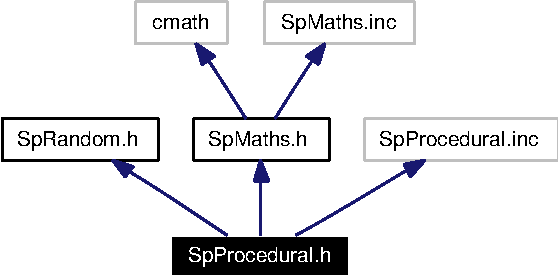
\includegraphics[width=151pt]{SpProcedural_8h__incl}
\end{center}
\end{figure}


This graph shows which files directly or indirectly include this file:\begin{figure}[H]
\begin{center}
\leavevmode
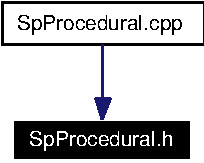
\includegraphics[width=66pt]{SpProcedural_8h__dep__incl}
\end{center}
\end{figure}
\subsection*{Namespaces}
\begin{CompactItemize}
\item 
namespace {\bf Spark}
\end{CompactItemize}
\subsection*{Functions}
\begin{CompactItemize}
\item 
template$<$class Real$>$ Real {\bf Quadric} (Real f\-A, Real f\-B, Real f\-C)
\item 
template$<$class Real$>$ Real {\bf Spline} (Real f\-X, unsigned int ui\-Knots, Real $\ast$apk\-Knots, const Real af\-B[4][4]=Catmull\-Rom\-Basis)
\item 
template$<$class Real$>$ Real {\bf Cell\-Noise} (Real f\-X, Real f\-Y, Real f\-Z)
\item 
template$<$class Real$>$ Real {\bf Gradient\-Noise} (Real f\-X, Real f\-Y, Real f\-Z)
\item 
template$<$class Real$>$ Real {\bf Value\-Noise} (Real f\-X, Real f\-Y, Real f\-Z, const Real af\-B[4][4]=Catmull\-Rom\-Basis)
\item 
template$<$class Real$>$ Real {\bf Fractional\-Brownian\-Motion} (Real f\-X, Real f\-Y, Real f\-Z, Real f\-Increment=0.5f, Real f\-Lacunarity=2.0345f, Real f\-Octaves=4.0f)
\item 
template$<$class Real$>$ Real {\bf Turbulence} (Real f\-X, Real f\-Y, Real f\-Z, Real f\-Increment=0.5f, Real f\-Lacunarity=2.0345f, Real f\-Octaves=4.0f)
\item 
template$<$class Real$>$ Real {\bf Mono\-Fractal} (Real f\-X, Real f\-Y, Real f\-Z, Real f\-Increment=0.5f, Real f\-Lacunarity=2.0345f, Real f\-Octaves=4.0f)
\item 
template$<$class Real$>$ Real {\bf Multi\-Fractal} (Real f\-X, Real f\-Y, Real f\-Z, Real f\-Increment=0.5f, Real f\-Lacunarity=2.0345f, Real f\-Octaves=4.0f)
\item 
template$<$class Real$>$ Real {\bf Hybrid\-Multi\-Fractal} (Real f\-X, Real f\-Y, Real f\-Z, Real f\-Increment=0.25f, Real f\-Lacunarity=2.0345f, Real f\-Offset=0.7f, Real f\-Gain=1.0f, Real f\-Octaves=4.0f)
\item 
template$<$class Real$>$ Real {\bf Ridged\-Multi\-Fractal} (Real f\-X, Real f\-Y, Real f\-Z, Real f\-Increment=0.9f, Real f\-Lacunarity=2.0345f, Real f\-Threshold=0.5f, Real f\-Offset=1.0f, Real f\-Octaves=4.0f)
\item 
template$<$class Real$>$ Real {\bf Filtered\-Turbulence} (Real f\-X, Real f\-Y, Real f\-Z, Real f\-Filter\-Width, Real f\-Increment=0.5f, Real f\-Lacunarity=2.0345f, Real f\-Octaves=4.0f)
\item 
template$<$class Real$>$ Real {\bf Filtered\-FBM} (Real f\-X, Real f\-Y, Real f\-Z, Real f\-Filter\-Width, Real f\-Increment=0.5f, Real f\-Lacunarity=2.0345f, Real f\-Octaves=4.0f)
\item 
template$<$class Real$>$ Real {\bf Voronoi\-Noise} (Real f\-X, Real f\-Y, Real f\-Z, Real f\-Jitter, Real \&rf\-OX, Real \&rf\-OY, Real \&rf\-OZ)
\item 
template$<$class Real$>$ Real {\bf Default\-Turbulence} (Real f\-X, Real f\-Y, Real f\-Z)
\item 
template$<$class Real$>$ Real {\bf Default\-FBM} (Real f\-X, Real f\-Y, Real f\-Z)
\item 
template$<$class Real$>$ Real {\bf Default\-Mono\-Fractal} (Real f\-X, Real f\-Y, Real f\-Z)
\item 
template$<$class Real$>$ Real {\bf Default\-Multi\-Fractal} (Real f\-X, Real f\-Y, Real f\-Z)
\item 
template$<$class Real$>$ Real {\bf Default\-Ridged\-Multi\-Fractal} (Real f\-X, Real f\-Y, Real f\-Z)
\item 
template$<$class Real$>$ Real {\bf f\-Bm} (Real f\-X, Real f\-Y, Real f\-Z, Real f\-Increment=0.5f, Real f\-Lacunarity=2.0345f, Real f\-Octaves=4.0f)
\item 
int {\bf p} (int i\-X)
\item 
float {\bf r} (int i\-X)
\item 
template$<$class Real$>$ int {\bf Hash} (int i\-X, int i\-Y, int i\-Z)
\item 
template$<$class Real$>$ Real {\bf Lattice} (int i\-X, int i\-Y, int i\-Z)
\item 
template$<$class Real$>$ Real {\bf Gradient} (int i\-X, int i\-Y, int i\-Z, Real f\-X, Real f\-Y, Real f\-Z)
\item 
template$<$class Real$>$ Real {\bf Bias} (Real f\-X, Real f\-A)
\item 
template$<$class Real$>$ Real {\bf Gain} (Real f\-X, Real f\-A)
\item 
template$<$class Real$>$ Real {\bf Cubic} (Real f\-T)
\item 
template$<$class Real$>$ Real {\bf Quintic} (Real f\-T)
\item 
template$<$class Real$>$ Real {\bf Lerp} (Real f\-T, Real f\-A, Real f\-B)
\item 
template$<$class Real$>$ Real {\bf Box\-Step} (Real f\-X, Real f\-A, Real f\-B)
\item 
template$<$class Real$>$ Real {\bf Smooth\-Step} (Real f\-A, Real f\-B, Real f\-X)
\item 
template$<$class Real$>$ Real {\bf Pulse} (Real f\-X, Real f\-A, Real f\-B)
\item 
template$<$class Real$>$ Real {\bf Box\-Pulse} (Real f\-X, Real f\-A, Real f\-B)
\item 
template$<$class Real$>$ Real {\bf Smooth\-Pulse} (Real f\-X, Real f\-A, Real f\-B)
\item 
template$<$class Real$>$ Real {\bf Filtered\-Abs} (Real f\-X, Real f\-DX)
\item 
template$<$class Real$>$ Real {\bf Catmull\-Rom\-Noise} (Real f\-X, Real f\-Y, Real f\-Z)
\item 
template$<$class Real$>$ Real {\bf Hermite\-Noise} (Real f\-X, Real f\-Y, Real f\-Z)
\item 
template$<$class Real$>$ Real {\bf Cardinal\-Noise} (Real f\-X, Real f\-Y, Real f\-Z)
\item 
template$<$class Real$>$ Real {\bf BSpline\-Noise} (Real f\-X, Real f\-Y, Real f\-Z)
\item 
template$<$class Real$>$ Real {\bf Filtered\-Gradient\-Noise} (Real f\-X, Real f\-Y, Real f\-Z, Real f\-Filter\-Width)
\end{CompactItemize}


\subsection{Function Documentation}
\index{SpProcedural.h@{Sp\-Procedural.h}!Bias@{Bias}}
\index{Bias@{Bias}!SpProcedural.h@{Sp\-Procedural.h}}
\subsubsection{\setlength{\rightskip}{0pt plus 5cm}template$<$class Real$>$ Real Spark::Bias (Real {\em f\-X}, Real {\em f\-A})}\label{namespaceSpark_a96}


Definition at line 261 of file Sp\-Procedural.h.\index{SpProcedural.h@{Sp\-Procedural.h}!BoxPulse@{BoxPulse}}
\index{BoxPulse@{BoxPulse}!SpProcedural.h@{Sp\-Procedural.h}}
\subsubsection{\setlength{\rightskip}{0pt plus 5cm}template$<$class Real$>$ Real Spark::Box\-Pulse (Real {\em f\-X}, Real {\em f\-A}, Real {\em f\-B})}\label{namespaceSpark_a104}


Definition at line 337 of file Sp\-Procedural.h.\index{SpProcedural.h@{Sp\-Procedural.h}!BoxStep@{BoxStep}}
\index{BoxStep@{BoxStep}!SpProcedural.h@{Sp\-Procedural.h}}
\subsubsection{\setlength{\rightskip}{0pt plus 5cm}template$<$class Real$>$ Real Spark::Box\-Step (Real {\em f\-X}, Real {\em f\-A}, Real {\em f\-B})}\label{namespaceSpark_a101}


Definition at line 311 of file Sp\-Procedural.h.\index{SpProcedural.h@{Sp\-Procedural.h}!BSplineNoise@{BSplineNoise}}
\index{BSplineNoise@{BSplineNoise}!SpProcedural.h@{Sp\-Procedural.h}}
\subsubsection{\setlength{\rightskip}{0pt plus 5cm}template$<$class Real$>$ Real Spark::BSpline\-Noise (Real {\em f\-X}, Real {\em f\-Y}, Real {\em f\-Z})}\label{namespaceSpark_a110}


Definition at line 362 of file Sp\-Procedural.h.\index{SpProcedural.h@{Sp\-Procedural.h}!CardinalNoise@{CardinalNoise}}
\index{CardinalNoise@{CardinalNoise}!SpProcedural.h@{Sp\-Procedural.h}}
\subsubsection{\setlength{\rightskip}{0pt plus 5cm}template$<$class Real$>$ Real Spark::Cardinal\-Noise (Real {\em f\-X}, Real {\em f\-Y}, Real {\em f\-Z})}\label{namespaceSpark_a109}


Definition at line 357 of file Sp\-Procedural.h.\index{SpProcedural.h@{Sp\-Procedural.h}!CatmullRomNoise@{CatmullRomNoise}}
\index{CatmullRomNoise@{CatmullRomNoise}!SpProcedural.h@{Sp\-Procedural.h}}
\subsubsection{\setlength{\rightskip}{0pt plus 5cm}template$<$class Real$>$ Real Spark::Catmull\-Rom\-Noise (Real {\em f\-X}, Real {\em f\-Y}, Real {\em f\-Z})}\label{namespaceSpark_a107}


Definition at line 347 of file Sp\-Procedural.h.\index{SpProcedural.h@{Sp\-Procedural.h}!CellNoise@{CellNoise}}
\index{CellNoise@{CellNoise}!SpProcedural.h@{Sp\-Procedural.h}}
\subsubsection{\setlength{\rightskip}{0pt plus 5cm}template$<$class Real$>$ Real Spark::Cell\-Noise (Real {\em f\-X}, Real {\em f\-Y}, Real {\em f\-Z})}\label{namespaceSpark_a73}


Definition at line 51 of file Sp\-Procedural.cpp.

References Spark::Floor(), Spark::Hash(), and Spark::r().

Referenced by Spark::Voronoi\-Noise().\index{SpProcedural.h@{Sp\-Procedural.h}!Cubic@{Cubic}}
\index{Cubic@{Cubic}!SpProcedural.h@{Sp\-Procedural.h}}
\subsubsection{\setlength{\rightskip}{0pt plus 5cm}template$<$class Real$>$ Real Spark::Cubic (Real {\em f\-T})}\label{namespaceSpark_a98}


Definition at line 291 of file Sp\-Procedural.h.

Referenced by Spark::Gradient\-Noise().\index{SpProcedural.h@{Sp\-Procedural.h}!DefaultFBM@{DefaultFBM}}
\index{DefaultFBM@{DefaultFBM}!SpProcedural.h@{Sp\-Procedural.h}}
\subsubsection{\setlength{\rightskip}{0pt plus 5cm}template$<$class Real$>$ Real Spark::Default\-FBM (Real {\em f\-X}, Real {\em f\-Y}, Real {\em f\-Z})}\label{namespaceSpark_a86}


Definition at line 395 of file Sp\-Procedural.h.\index{SpProcedural.h@{Sp\-Procedural.h}!DefaultMonoFractal@{DefaultMonoFractal}}
\index{DefaultMonoFractal@{DefaultMonoFractal}!SpProcedural.h@{Sp\-Procedural.h}}
\subsubsection{\setlength{\rightskip}{0pt plus 5cm}template$<$class Real$>$ Real Spark::Default\-Mono\-Fractal (Real {\em f\-X}, Real {\em f\-Y}, Real {\em f\-Z})}\label{namespaceSpark_a87}


Definition at line 401 of file Sp\-Procedural.h.\index{SpProcedural.h@{Sp\-Procedural.h}!DefaultMultiFractal@{DefaultMultiFractal}}
\index{DefaultMultiFractal@{DefaultMultiFractal}!SpProcedural.h@{Sp\-Procedural.h}}
\subsubsection{\setlength{\rightskip}{0pt plus 5cm}template$<$class Real$>$ Real Spark::Default\-Multi\-Fractal (Real {\em f\-X}, Real {\em f\-Y}, Real {\em f\-Z})}\label{namespaceSpark_a88}


Definition at line 407 of file Sp\-Procedural.h.\index{SpProcedural.h@{Sp\-Procedural.h}!DefaultRidgedMultiFractal@{DefaultRidgedMultiFractal}}
\index{DefaultRidgedMultiFractal@{DefaultRidgedMultiFractal}!SpProcedural.h@{Sp\-Procedural.h}}
\subsubsection{\setlength{\rightskip}{0pt plus 5cm}template$<$class Real$>$ Real Spark::Default\-Ridged\-Multi\-Fractal (Real {\em f\-X}, Real {\em f\-Y}, Real {\em f\-Z})}\label{namespaceSpark_a89}


Definition at line 413 of file Sp\-Procedural.h.\index{SpProcedural.h@{Sp\-Procedural.h}!DefaultTurbulence@{DefaultTurbulence}}
\index{DefaultTurbulence@{DefaultTurbulence}!SpProcedural.h@{Sp\-Procedural.h}}
\subsubsection{\setlength{\rightskip}{0pt plus 5cm}template$<$class Real$>$ Real Spark::Default\-Turbulence (Real {\em f\-X}, Real {\em f\-Y}, Real {\em f\-Z})}\label{namespaceSpark_a85}


Definition at line 389 of file Sp\-Procedural.h.\index{SpProcedural.h@{Sp\-Procedural.h}!fBm@{fBm}}
\index{fBm@{fBm}!SpProcedural.h@{Sp\-Procedural.h}}
\subsubsection{\setlength{\rightskip}{0pt plus 5cm}template$<$class Real$>$ Real Spark::f\-Bm (Real {\em f\-X}, Real {\em f\-Y}, Real {\em f\-Z}, Real {\em f\-Increment} = {\tt 0.5f}, Real {\em f\-Lacunarity} = {\tt 2.0345f}, Real {\em f\-Octaves} = {\tt 4.0f})}\label{namespaceSpark_a90}


Definition at line 419 of file Sp\-Procedural.h.\index{SpProcedural.h@{Sp\-Procedural.h}!FilteredAbs@{FilteredAbs}}
\index{FilteredAbs@{FilteredAbs}!SpProcedural.h@{Sp\-Procedural.h}}
\subsubsection{\setlength{\rightskip}{0pt plus 5cm}template$<$class Real$>$ Real Spark::Filtered\-Abs (Real {\em f\-X}, Real {\em f\-DX})}\label{namespaceSpark_a106}


Definition at line 367 of file Sp\-Procedural.h.

Referenced by Spark::Filtered\-Turbulence().\index{SpProcedural.h@{Sp\-Procedural.h}!FilteredFBM@{FilteredFBM}}
\index{FilteredFBM@{FilteredFBM}!SpProcedural.h@{Sp\-Procedural.h}}
\subsubsection{\setlength{\rightskip}{0pt plus 5cm}template$<$class Real$>$ Real Spark::Filtered\-FBM (Real {\em f\-X}, Real {\em f\-Y}, Real {\em f\-Z}, Real {\em f\-Filter\-Width}, Real {\em f\-Increment} = {\tt 0.5f}, Real {\em f\-Lacunarity} = {\tt 2.0345f}, Real {\em f\-Octaves} = {\tt 4.0f})}\label{namespaceSpark_a83}


Definition at line 188 of file Sp\-Procedural.cpp.

References Spark::Filtered\-Gradient\-Noise().\index{SpProcedural.h@{Sp\-Procedural.h}!FilteredGradientNoise@{FilteredGradientNoise}}
\index{FilteredGradientNoise@{FilteredGradientNoise}!SpProcedural.h@{Sp\-Procedural.h}}
\subsubsection{\setlength{\rightskip}{0pt plus 5cm}template$<$class Real$>$ Real Spark::Filtered\-Gradient\-Noise (Real {\em f\-X}, Real {\em f\-Y}, Real {\em f\-Z}, Real {\em f\-Filter\-Width})}\label{namespaceSpark_a111}


Definition at line 382 of file Sp\-Procedural.h.

Referenced by Spark::Filtered\-FBM(), and Spark::Filtered\-Turbulence().\index{SpProcedural.h@{Sp\-Procedural.h}!FilteredTurbulence@{FilteredTurbulence}}
\index{FilteredTurbulence@{FilteredTurbulence}!SpProcedural.h@{Sp\-Procedural.h}}
\subsubsection{\setlength{\rightskip}{0pt plus 5cm}template$<$class Real$>$ Real Spark::Filtered\-Turbulence (Real {\em f\-X}, Real {\em f\-Y}, Real {\em f\-Z}, Real {\em f\-Filter\-Width}, Real {\em f\-Increment} = {\tt 0.5f}, Real {\em f\-Lacunarity} = {\tt 2.0345f}, Real {\em f\-Octaves} = {\tt 4.0f})}\label{namespaceSpark_a82}


Definition at line 296 of file Sp\-Procedural.cpp.

References Spark::Filtered\-Abs(), and Spark::Filtered\-Gradient\-Noise().\index{SpProcedural.h@{Sp\-Procedural.h}!FractionalBrownianMotion@{FractionalBrownianMotion}}
\index{FractionalBrownianMotion@{FractionalBrownianMotion}!SpProcedural.h@{Sp\-Procedural.h}}
\subsubsection{\setlength{\rightskip}{0pt plus 5cm}template$<$class Real$>$ Real Spark::Fractional\-Brownian\-Motion (Real {\em f\-X}, Real {\em f\-Y}, Real {\em f\-Z}, Real {\em f\-Increment} = {\tt 0.5f}, Real {\em f\-Lacunarity} = {\tt 2.0345f}, Real {\em f\-Octaves} = {\tt 4.0f})}\label{namespaceSpark_a76}


Definition at line 143 of file Sp\-Procedural.cpp.

References Spark::Gradient\-Noise().\index{SpProcedural.h@{Sp\-Procedural.h}!Gain@{Gain}}
\index{Gain@{Gain}!SpProcedural.h@{Sp\-Procedural.h}}
\subsubsection{\setlength{\rightskip}{0pt plus 5cm}template$<$class Real$>$ Real Spark::Gain (Real {\em f\-X}, Real {\em f\-A})}\label{namespaceSpark_a97}


Definition at line 270 of file Sp\-Procedural.h.\index{SpProcedural.h@{Sp\-Procedural.h}!Gradient@{Gradient}}
\index{Gradient@{Gradient}!SpProcedural.h@{Sp\-Procedural.h}}
\subsubsection{\setlength{\rightskip}{0pt plus 5cm}template$<$class Real$>$ Real Spark::Gradient (int {\em i\-X}, int {\em i\-Y}, int {\em i\-Z}, Real {\em f\-X}, Real {\em f\-Y}, Real {\em f\-Z})}\label{namespaceSpark_a95}


Definition at line 241 of file Sp\-Procedural.h.

Referenced by Spark::Gradient\-Noise().\index{SpProcedural.h@{Sp\-Procedural.h}!GradientNoise@{GradientNoise}}
\index{GradientNoise@{GradientNoise}!SpProcedural.h@{Sp\-Procedural.h}}
\subsubsection{\setlength{\rightskip}{0pt plus 5cm}template$<$class Real$>$ Real Spark::Gradient\-Noise (Real {\em f\-X}, Real {\em f\-Y}, Real {\em f\-Z})}\label{namespaceSpark_a74}


Definition at line 61 of file Sp\-Procedural.cpp.

References Spark::Cubic(), Spark::Floor(), Spark::Gradient(), and Spark::Lerp().

Referenced by Spark::Fractional\-Brownian\-Motion(), Spark::Hybrid\-Multi\-Fractal(), Spark::Mono\-Fractal(), Spark::Multi\-Fractal(), Spark::Ridged\-Multi\-Fractal(), and Spark::Turbulence().\index{SpProcedural.h@{Sp\-Procedural.h}!Hash@{Hash}}
\index{Hash@{Hash}!SpProcedural.h@{Sp\-Procedural.h}}
\subsubsection{\setlength{\rightskip}{0pt plus 5cm}template$<$class Real$>$ int Spark::Hash (int {\em i\-X}, int {\em i\-Y}, int {\em i\-Z})}\label{namespaceSpark_a93}


Definition at line 231 of file Sp\-Procedural.h.

Referenced by Spark::Cell\-Noise().\index{SpProcedural.h@{Sp\-Procedural.h}!HermiteNoise@{HermiteNoise}}
\index{HermiteNoise@{HermiteNoise}!SpProcedural.h@{Sp\-Procedural.h}}
\subsubsection{\setlength{\rightskip}{0pt plus 5cm}template$<$class Real$>$ Real Spark::Hermite\-Noise (Real {\em f\-X}, Real {\em f\-Y}, Real {\em f\-Z})}\label{namespaceSpark_a108}


Definition at line 352 of file Sp\-Procedural.h.\index{SpProcedural.h@{Sp\-Procedural.h}!HybridMultiFractal@{HybridMultiFractal}}
\index{HybridMultiFractal@{HybridMultiFractal}!SpProcedural.h@{Sp\-Procedural.h}}
\subsubsection{\setlength{\rightskip}{0pt plus 5cm}template$<$class Real$>$ Real Spark::Hybrid\-Multi\-Fractal (Real {\em f\-X}, Real {\em f\-Y}, Real {\em f\-Z}, Real {\em f\-Increment} = {\tt 0.25f}, Real {\em f\-Lacunarity} = {\tt 2.0345f}, Real {\em f\-Offset} = {\tt 0.7f}, Real {\em f\-Gain} = {\tt 1.0f}, Real {\em f\-Octaves} = {\tt 4.0f})}\label{namespaceSpark_a80}


Definition at line 456 of file Sp\-Procedural.cpp.

References Spark::Gradient\-Noise().\index{SpProcedural.h@{Sp\-Procedural.h}!Lattice@{Lattice}}
\index{Lattice@{Lattice}!SpProcedural.h@{Sp\-Procedural.h}}
\subsubsection{\setlength{\rightskip}{0pt plus 5cm}template$<$class Real$>$ Real Spark::Lattice (int {\em i\-X}, int {\em i\-Y}, int {\em i\-Z})}\label{namespaceSpark_a94}


Definition at line 236 of file Sp\-Procedural.h.

Referenced by Spark::Value\-Noise().\index{SpProcedural.h@{Sp\-Procedural.h}!Lerp@{Lerp}}
\index{Lerp@{Lerp}!SpProcedural.h@{Sp\-Procedural.h}}
\subsubsection{\setlength{\rightskip}{0pt plus 5cm}template$<$class Real$>$ Real Spark::Lerp (Real {\em f\-T}, Real {\em f\-A}, Real {\em f\-B})}\label{namespaceSpark_a100}


Definition at line 301 of file Sp\-Procedural.h.

Referenced by Spark::Gradient\-Noise().\index{SpProcedural.h@{Sp\-Procedural.h}!MonoFractal@{MonoFractal}}
\index{MonoFractal@{MonoFractal}!SpProcedural.h@{Sp\-Procedural.h}}
\subsubsection{\setlength{\rightskip}{0pt plus 5cm}template$<$class Real$>$ Real Spark::Mono\-Fractal (Real {\em f\-X}, Real {\em f\-Y}, Real {\em f\-Z}, Real {\em f\-Increment} = {\tt 0.5f}, Real {\em f\-Lacunarity} = {\tt 2.0345f}, Real {\em f\-Octaves} = {\tt 4.0f})}\label{namespaceSpark_a78}


Definition at line 356 of file Sp\-Procedural.cpp.

References Spark::Gradient\-Noise().\index{SpProcedural.h@{Sp\-Procedural.h}!MultiFractal@{MultiFractal}}
\index{MultiFractal@{MultiFractal}!SpProcedural.h@{Sp\-Procedural.h}}
\subsubsection{\setlength{\rightskip}{0pt plus 5cm}template$<$class Real$>$ Real Spark::Multi\-Fractal (Real {\em f\-X}, Real {\em f\-Y}, Real {\em f\-Z}, Real {\em f\-Increment} = {\tt 0.5f}, Real {\em f\-Lacunarity} = {\tt 2.0345f}, Real {\em f\-Octaves} = {\tt 4.0f})}\label{namespaceSpark_a79}


Definition at line 407 of file Sp\-Procedural.cpp.

References Spark::Gradient\-Noise().\index{SpProcedural.h@{Sp\-Procedural.h}!p@{p}}
\index{p@{p}!SpProcedural.h@{Sp\-Procedural.h}}
\subsubsection{\setlength{\rightskip}{0pt plus 5cm}int Spark::p (int {\em i\-X})\hspace{0.3cm}{\tt  [inline]}}\label{namespaceSpark_a91}


Definition at line 225 of file Sp\-Procedural.h.\index{SpProcedural.h@{Sp\-Procedural.h}!Pulse@{Pulse}}
\index{Pulse@{Pulse}!SpProcedural.h@{Sp\-Procedural.h}}
\subsubsection{\setlength{\rightskip}{0pt plus 5cm}template$<$class Real$>$ Real Spark::Pulse (Real {\em f\-X}, Real {\em f\-A}, Real {\em f\-B})}\label{namespaceSpark_a103}


Definition at line 332 of file Sp\-Procedural.h.\index{SpProcedural.h@{Sp\-Procedural.h}!Quadric@{Quadric}}
\index{Quadric@{Quadric}!SpProcedural.h@{Sp\-Procedural.h}}
\subsubsection{\setlength{\rightskip}{0pt plus 5cm}template$<$class Real$>$ Real Spark::Quadric (Real {\em f\-A}, Real {\em f\-B}, Real {\em f\-C})}\label{namespaceSpark_a71}


Definition at line 598 of file Sp\-Procedural.cpp.

References Spark::Sqrt().\index{SpProcedural.h@{Sp\-Procedural.h}!Quintic@{Quintic}}
\index{Quintic@{Quintic}!SpProcedural.h@{Sp\-Procedural.h}}
\subsubsection{\setlength{\rightskip}{0pt plus 5cm}template$<$class Real$>$ Real Spark::Quintic (Real {\em f\-T})}\label{namespaceSpark_a99}


Definition at line 296 of file Sp\-Procedural.h.\index{SpProcedural.h@{Sp\-Procedural.h}!r@{r}}
\index{r@{r}!SpProcedural.h@{Sp\-Procedural.h}}
\subsubsection{\setlength{\rightskip}{0pt plus 5cm}float Spark::r (int {\em i\-X})\hspace{0.3cm}{\tt  [inline]}}\label{namespaceSpark_a92}


Definition at line 219 of file Sp\-Procedural.h.

Referenced by Spark::Cell\-Noise().\index{SpProcedural.h@{Sp\-Procedural.h}!RidgedMultiFractal@{RidgedMultiFractal}}
\index{RidgedMultiFractal@{RidgedMultiFractal}!SpProcedural.h@{Sp\-Procedural.h}}
\subsubsection{\setlength{\rightskip}{0pt plus 5cm}template$<$class Real$>$ Real Spark::Ridged\-Multi\-Fractal (Real {\em f\-X}, Real {\em f\-Y}, Real {\em f\-Z}, Real {\em f\-Increment} = {\tt 0.9f}, Real {\em f\-Lacunarity} = {\tt 2.0345f}, Real {\em f\-Threshold} = {\tt 0.5f}, Real {\em f\-Offset} = {\tt 1.0f}, Real {\em f\-Octaves} = {\tt 4.0f})}\label{namespaceSpark_a81}


Definition at line 527 of file Sp\-Procedural.cpp.

References Spark::Abs(), Spark::Clamp(), and Spark::Gradient\-Noise().\index{SpProcedural.h@{Sp\-Procedural.h}!SmoothPulse@{SmoothPulse}}
\index{SmoothPulse@{SmoothPulse}!SpProcedural.h@{Sp\-Procedural.h}}
\subsubsection{\setlength{\rightskip}{0pt plus 5cm}template$<$class Real$>$ Real Spark::Smooth\-Pulse (Real {\em f\-X}, Real {\em f\-A}, Real {\em f\-B})}\label{namespaceSpark_a105}


Definition at line 342 of file Sp\-Procedural.h.\index{SpProcedural.h@{Sp\-Procedural.h}!SmoothStep@{SmoothStep}}
\index{SmoothStep@{SmoothStep}!SpProcedural.h@{Sp\-Procedural.h}}
\subsubsection{\setlength{\rightskip}{0pt plus 5cm}template$<$class Real$>$ Real Spark::Smooth\-Step (Real {\em f\-A}, Real {\em f\-B}, Real {\em f\-X})}\label{namespaceSpark_a102}


Definition at line 316 of file Sp\-Procedural.h.\index{SpProcedural.h@{Sp\-Procedural.h}!Spline@{Spline}}
\index{Spline@{Spline}!SpProcedural.h@{Sp\-Procedural.h}}
\subsubsection{\setlength{\rightskip}{0pt plus 5cm}template$<$class Real$>$ Real Spark::Spline (Real {\em f\-X}, unsigned int {\em ui\-Knots}, Real $\ast$ {\em apk\-Knots}, const Real {\em af\-B}[4][4] = {\tt CatmullRomBasis})}\label{namespaceSpark_a72}


Definition at line 28 of file Sp\-Procedural.cpp.

References Spark::Clamp().

Referenced by Spark::Value\-Noise().\index{SpProcedural.h@{Sp\-Procedural.h}!Turbulence@{Turbulence}}
\index{Turbulence@{Turbulence}!SpProcedural.h@{Sp\-Procedural.h}}
\subsubsection{\setlength{\rightskip}{0pt plus 5cm}template$<$class Real$>$ Real Spark::Turbulence (Real {\em f\-X}, Real {\em f\-Y}, Real {\em f\-Z}, Real {\em f\-Increment} = {\tt 0.5f}, Real {\em f\-Lacunarity} = {\tt 2.0345f}, Real {\em f\-Octaves} = {\tt 4.0f})}\label{namespaceSpark_a77}


Definition at line 238 of file Sp\-Procedural.cpp.

References Spark::Abs(), and Spark::Gradient\-Noise().\index{SpProcedural.h@{Sp\-Procedural.h}!ValueNoise@{ValueNoise}}
\index{ValueNoise@{ValueNoise}!SpProcedural.h@{Sp\-Procedural.h}}
\subsubsection{\setlength{\rightskip}{0pt plus 5cm}template$<$class Real$>$ Real Spark::Value\-Noise (Real {\em f\-X}, Real {\em f\-Y}, Real {\em f\-Z}, const Real {\em af\-B}[4][4] = {\tt CatmullRomBasis})}\label{namespaceSpark_a75}


Definition at line 111 of file Sp\-Procedural.cpp.

References Spark::Lattice(), and Spark::Spline().\index{SpProcedural.h@{Sp\-Procedural.h}!VoronoiNoise@{VoronoiNoise}}
\index{VoronoiNoise@{VoronoiNoise}!SpProcedural.h@{Sp\-Procedural.h}}
\subsubsection{\setlength{\rightskip}{0pt plus 5cm}template$<$class Real$>$ Real Spark::Voronoi\-Noise (Real {\em f\-X}, Real {\em f\-Y}, Real {\em f\-Z}, Real {\em f\-Jitter}, Real \& {\em rf\-OX}, Real \& {\em rf\-OY}, Real \& {\em rf\-OZ})}\label{namespaceSpark_a84}


Definition at line 625 of file Sp\-Procedural.cpp.

References Spark::Cell\-Noise(), Spark::Floor(), and Spark::Sqrt().